\documentclass[10pt,a4paper]{jarticle}
%\pagestyle{empty}%ページ非表示
%usepackage{fancyhdr}%ヘッダ
\usepackage[dvipdfmx]{graphicx}%画像
\usepackage{moreverb}
\renewcommand{\figurename}{図}
\renewcommand{\tablenema}{表}
\begin{document}
%ここから
\title{H8マイコンによるステッピングモータ制御}
\author{筒居 稔}
\maketitle
%\lhead{左ヘッダ}
%\chead{中央ヘッダ}
%\rhead{右ヘッダ}
%\part*{部}
%\chapter*{章}
\section{実験目的}
産業用ロボットの関節,ハードディスクのヘッド移動、X-Yステージの台座など、
制度の要求される位置決めアクチュエータとして重要な
ステッピングモータについて理解する。
ステッピングモータは、複数のチャンネルによるパルスの組み合わせにより制御するため、
デジタル制御回路との相性がいい。
そこで、C言語によりプログラム開発を行い、H8マイコンを用いて
ステッピングモータを制御する方法を習得する。
%\subsection*{小節}
%\subsubsection*{少々節}
\section{実験機器}
\begin{table}[hbtp]
 \caption{使用機器}
 \label{siyou}
 \centering
  \begin{tabular}{|c|c|c|}\hline
  機器名&メーカー&製品名\\ \hline
  ステッピングモータ&日本電産コパル&SPG27-1601\\ \hline
  H8マイコン&ルネサスエレクトロニクス&H8/3052F\\ \hline
  直流安定化電源&GW Instek&GPS-1805D\\ \hline
  オシロスコープ&GW Instek&GDS-1052-U\\ \hline
  \end{tabular}
\end{table}
\section{実験原理}
\subsection{ステッピングモータの動作原理}
ステッピングモータはパルスモータとも呼ばれ、
パルス信号を与えることにより決められたステップ単位で回転する。\par
\begin{figure}[hbtp]
 \centering
  \fbox{\includegraphics[scale=0.8]{/home/minoru/Desktop/tex/h82pic/XC16082.eps}}
 \caption{ステッピングモータの構成}
 \label{fig:step}
\end{figure}
図1は今回使用した
二相のユニポーラ型ステッピングモータの構成である。
図1内のφ1Cとφ2Cはそれぞれ電源とつながり、
それ以外はグランドとつながっている。
φ1Cからφ1、φ2Cからφ2、
φ1Cから\overline{φ1}、φ2Cから\overline{φ2}の順に
電流を流す(励磁する)とモータが回転する。
\subsection{1相励磁と2相励磁}
ステッピングモータにパルス信号を送る際に、
1相励磁の場合、φ1、φ2、\overline{φ1}、\overline{φ2}、
と順に信号を送ればモータは回転する。
2相励磁の場合はパルスを送る順番は1相励磁と同じだかが、
前に送った信号と次に送る信号に半分ずつ
今回の信号をかぶせてモータの回転をなめらかにする。
\section{実験方法}
\subsection{SCI通信実験}
自身のPCでGCC Developer Liteを管理者モードで起動し、設定をもう一度確認する。
ソースコード1を記述し、メニューの「コンパイル」「ビルド」でコンパイルする。
エラーが出た場合はミスを直し再びコンパイルする。\par
エラーが出ず、コンパイルに成功した場合
以下の手順でプログラムの書き込みを行う。\par
\begin{enumerate}
 \item USBシリアル変換ケーブルをPCに接続し、
 デバイスマネージャーでCOM番号を確認する。
 \item シリアルケーブルを実習装置側のSCIコネクタに接続する。
 \item 書き込みスイッチをONにし、モード設定端子のMD2をジャンパピンで短絡させる
 \item マイコンボードの電源コネクタにACアダプタを接続する。(緑色LEDが点灯)
 \item H8 Writerを起動し、書き込み制御ファイルを「3052\_F25M\_P384.MOT」、
 Baud(B)を「19200」、Baund(P)を「38400」にした後、
 COM Portを自分のパソコンに合わせる。
 \item 「書き込むファイル」をクリックし、書き込みたいファイル
 (作成したソースコードの拡張子をmotにしたもの)を指定する。
 最後に「書き込み開始」をクリックすると書き込みが始まる。
 \item 書き込みが完了したら、ACアダプタを外してから、
 書き込みスイッチをOFFにし、モード設定端子のジャンパピンを
 MD2からMD0に付け替える。
\end{enumerate}
そして「ツール」からSIMLE TERMを立ち上げ、「ファイル」「プロパティ」を開き、
PropatyのConnect toを自分の設定に、Baudrateを「38400」に合わせ、
「通信」「ポートオープン」を選択する。\par
マイコンボードにACアダプタを接続すると、ターミナルに「@」が表示され、
キー入力すると、その文字が表示されることを確認。
確認後、ACアダプタを外す。
\subsection{ステッピングモータの手動動作実験}
\subsubsection{未完成部分の接続}
\begin{enumerate}
 \item 図1を参考にモータドライバ回路と、ステッピングモータを接続。
 \item モータ用電源に外部電源を接続。
 \item マイコンボードにACアダプタを接続する。
 \item 外部電源を5Vに設定し電圧を印加する。
\end{enumerate}
\subsubsection{手動動作確認}
\begin{enumerate}
 \item 0から3のスイッチを順番に押し、モータが回転することを確認する。
 \item 3から0のスイッチを順番に押し、モータが逆回転することを確認する。
 \item スイッチのON/OFFとトランジスタの状態、
 およびステッピングモータの励磁状態をまとめる。
\end{enumerate}
\subsection{ステッピングモータのマイコン制御実験}
\subsubsection{正回転動作の確認}
\begin{enumerate}
 \item \verb|program/stopmotor3052.c|をコンパイルし、マイコンに書き込む。
 \item モータ用電源に外部電源で5Vを印加する。
 \item SIMPLE TERMを起動し、マイコンボードにACアダプタを接続する。
 \item 「g」キーを入力すると正回転することを確認する。
 \item 「g」キー以外を入力すると回転が停止することを確認する。
\end{enumerate}
\subsubsection{モータ印加電圧による回転速度変化の確認}
\begin{enumerate}
 \item モータ用電源に外部電源で5Vを印加した状態で、
 1回転に要する時間を測定する。
 \item 印加電圧を9V、12Vに変化させ、同時に時間を測定する。
\end{enumerate}
\subsubsection{1相励磁と2相励磁による回転速度とスムーズさの確認}
\begin{enumerate}
 \item プログラムを変更し、小文字の「g」で1相励磁、
 「j」で2相励磁となるようにする。
 \item それぞれの相で回転速度を確認する。そのとき目視で動作の状態を確認する。
 \item それぞれの相での波形状態をオシロスコープで確認する。
\end{enumerate}
\subsubsection{正回転、逆回転動作の確認}
\begin{enumerate}
 \item プログラムを変更し、「g」で正回転、
 「h」で逆回転動作となるようにする。
 \item 動作を目視で確認し、オシロスコープで波形確認する。
\end{enumerate}
\section{実験結果}
\subsection{SCI通信実験}
ソースコードでコンパイル後手順に従い書き込み、通信を確認。
\subsection{ステッピングモータの手動動作実験}
\subsubsection{未完部分の接続}
図1に従いモータと回路を接続。
\subsubsection{手動操作確認}
スイッチを順番に押し回転、逆回転を確認。
\subsection{ステッピングモータのマイコン制御実験}
\subsubsection{正回転動作の確認}
ソースコード2を入力後正回転を確認。
\subsubsection{モータ印加電圧による回転速度変化の確認}
直流安定化電源を用いて、印加電圧を5V、9V、12V
と変化させモータの回転速度の変化を目視で確認。\par
\begin{table}[htbp]
 \caption{印加電圧によるモータの1回転に要する時間の変化}
 \label{denatu}
 \centering
 \begin{tabular}{|r|r|}\hline
   電圧[V]&時間[s]\\ \hline
   4.99[V]&0.0[s]\\ \hline
   9.00[V]&12.5[s]\\ \hline
   12.00[V]&11.9[s]\\ \hline
   15.00[v]&11.8[s]\\ \hline
 \end{tabular}
\end{table}
\subsubsection{1相励磁と2相励磁による回転速度とスムーズさの確認}
ソースコード3を入力後「g」で1相励磁「j」で2相励磁で
ステップモータを回転させ、回転状態を目視で確認。
目視では違いを確認できなかった。
オシロスコープで1相励磁と2相励磁の波形を取った
\begin{figure}[hbtp]
 \begin{minipage}{0.5\hsize}
 \begin{center}
  \fbox{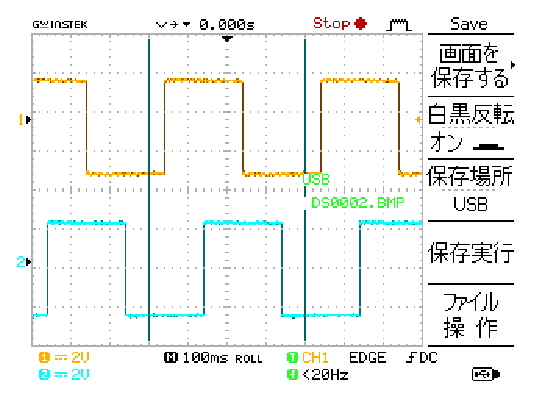
\includegraphics[scale=0.6]{/home/minoru/Desktop/tex/h82pic/no5/DS0002.eps}}
 \caption{2相励磁}
 \label{fig:2rei}
 \end{center}
 \end{minipage}
 \begin{minipage}{0.5\hsize}
 \begin{center}
  \fbox{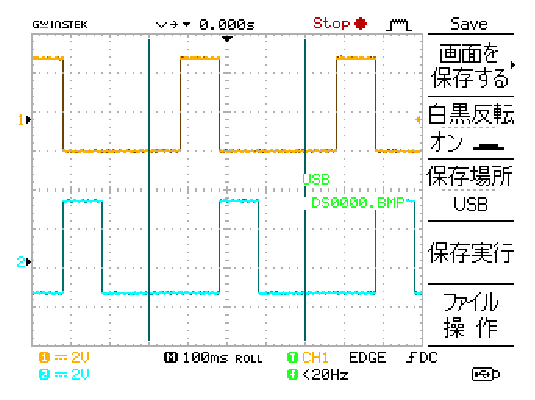
\includegraphics[scale=0.6]{/home/minoru/Desktop/tex/h82pic/no5/DS0000.eps}}
 \caption{1相励磁}
 \label{fig:1rei}
 \end{center}
 \end{minipage}
\end{figure}
\subsubsection{正回転、逆回転動作の確認}
ソースコード3を入力後「g」で正回転、「h」で逆回転を確認。
オシロスコープで波形を取った。
\begin{figure}[hbtp]
 \begin{center}
  \fbox{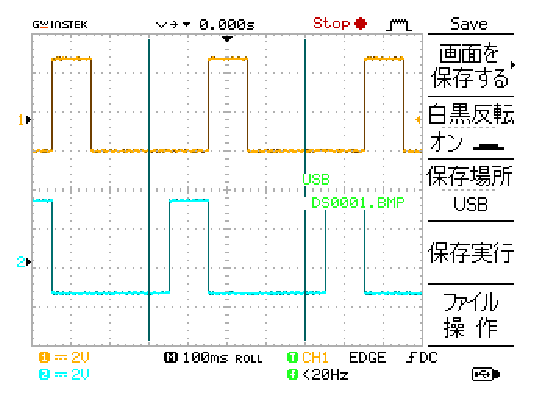
\includegraphics[scale=0.6]{/home/minoru/Desktop/tex/h82pic/no5/DS0001.eps}}
 \caption{逆回転}
 \label{fig:gyaku}
 \end{center}
\end{figure}
\section{ソースコード}

\section{考察}
印加電圧によるモータの1回転に要する時間の変化では、
5Vでは回転しなかったが、9〜15Vでは時間に差はあったものの、小さかった。
計測時間の差は誤差であり、
印加電圧の差によりモータの1回転に要する時間は変化しない、
なぜならステッピングモータの回転速度は
与えられたパルス信号により変化するからである。
しかし印加電圧が上がればモータのトルクは上がる。\par
ステッピングモータ制御のプログラムでは、
マイコンとの通信により、キーボドから入力された値を検出し、
{\small
\begin{verbatim}
  case 'g':
    if(fst) { sci_print("  g\n"); fst = 0; }
    switch(cnt) {
    case 0: PB.DR.BYTE = 0b0001; break;
    case 1: PB.DR.BYTE = 0b0010; break;
    case 2: PB.DR.BYTE = 0b0100; break;
    case 3: PB.DR.BYTE = 0b1000; break;
    }
\end{verbatim}
}
をループさせることにより制御している。
この際、マイコンのポートに信号を送っているのは
{\small
\begin{verbatim}
0bxxxx(xは0か1)
\end{verbatim}
}
の部分であり、xが0か1かでステッピングモータのφ1、φ2、
\overline{φ1}、\overline{φ2}にパルス信号を送るか決める。
そのため逆回転では正回転のパルス信号を
反転させた信号を送信した。
2相励磁では前回と次回のパルス信号に
自身の信号が半分かぶれば良いため
前後の相と1パルス文ずらしながら同時に励磁させた。
1相励磁と2相励磁の違いは目視では確認できなかったが、
実際には2相励磁では、パルス幅が1相励磁の2倍となり、
1相励磁に比べて回転が安定し、大きなトルクが得られる、
ただし消費電力も二倍となる。
%ここまで
\end{document}
